\documentclass[11pt]{article}
\usepackage[margin=1in]{geometry}
\usepackage{amsmath,amssymb,amsthm}
\usepackage{algorithm}
\usepackage{algpseudocode}
\usepackage{booktabs}
\usepackage{hyperref}
\usepackage{tikz}
\usetikzlibrary{positioning,shapes.geometric,shapes.misc}

\newtheorem{definition}{Definition}
\newtheorem{theorem}{Theorem}
\newtheorem{proposition}{Proposition}
\newtheorem{example}{Example}

\title{Mean-Field Variational Inference\\for Credal Networks}
\author{IBM Research}
\date{}

\begin{document}
\maketitle

\begin{abstract}
We describe a mean-field variational inference algorithm for credal networks that
computes bounds on marginal probabilities by exploring combinations of extreme points
from the local credal sets. For each selected combination of extreme points, the
credal network reduces to a standard Bayesian network on which classical mean-field
coordinate ascent is applied. By tracking the minimum and maximum of the variational
distribution across all explored combinations, the algorithm produces probability
intervals for the query variable. This approach complements the interval belief
propagation method by providing an alternative view of the credal inference problem
through the lens of variational optimization.
\end{abstract}

\section{Preliminaries}

\subsection{Mean-Field Variational Inference}

Given a probability distribution $P(\mathbf{X})$ that factorizes according to a
Bayesian network, the \textbf{mean-field} approximation seeks a factored distribution
$q(\mathbf{X}) = \prod_{i=1}^n q_i(X_i)$ that minimizes the KL divergence:
\begin{equation}\label{eq:kl}
  \mathrm{KL}(q \| P) = \sum_{\mathbf{x}} q(\mathbf{x}) \log \frac{q(\mathbf{x})}{P(\mathbf{x})}.
\end{equation}

The optimal update for each factor $q_i(X_i)$ is:
\begin{equation}\label{eq:mf-update}
  \log q_i^*(X_i) = \mathbb{E}_{q_{\setminus i}}\bigl[\log P(\mathbf{X})\bigr] + \mathrm{const},
\end{equation}
where $q_{\setminus i}$ denotes the product of all factors except $q_i$.

For a Bayesian network $P(\mathbf{X}) = \prod_i P(X_i \mid \mathrm{Pa}(X_i))$,
Equation~\eqref{eq:mf-update} decomposes into contributions from the local CPTs
involving $X_i$ (either as child or parent):
\begin{equation}\label{eq:mf-bn}
  \log q_i^*(X_i = x) = \sum_{f : X_i \in \mathrm{scope}(f)}
  \mathbb{E}_{q_{\setminus i}}\bigl[\log P_f \bigr],
\end{equation}
where $P_f$ denotes the CPT of factor $f$ evaluated at the relevant configuration.

\subsection{Extension to Credal Networks}

In a credal network, each local CPT $P(X_i \mid \mathrm{Pa}(X_i))$ is not a single
distribution but a member of a credal set $K(X_i \mid \mathrm{Pa}(X_i))$.
The strong extension is the convex hull of all joint distributions formed by selecting
one extreme point per local credal set:
\begin{equation}\label{eq:strong-ext}
  \mathrm{co}\,K(\mathbf{X}) = \mathrm{CH}\Bigl\{
    \prod_{i} P(X_i \mid \pi_i) : P(X_i \mid \pi_i) \in \mathrm{ext}\,K(X_i \mid \pi_i)
  \Bigr\}.
\end{equation}

Our approach exploits this structure: for each combination of extreme points (one per
local credal set per parent configuration), we obtain a standard Bayesian network.
Running mean-field variational inference on this BN produces a specific $q(\mathbf{X})$.
By tracking the range of $q(Z)$ across all explored combinations, we obtain bounds
on $P(Z \mid \mathbf{Y} = \mathbf{y})$.

\section{Vertex Combinations in Detail}\label{sec:vc}

Each factor $f_i$ in the credal network (associated with node $X_i$ and parents
$\mathrm{Pa}(X_i)$) stores a credal set $K(X_i \mid \pi)$ for each parent
configuration $\pi$. Each credal set has extreme points:
\[
  \mathrm{ext}\,K(X_i \mid \pi) = \{P_1(X_i \mid \pi),\; \dots,\; P_{n_\pi}(X_i \mid \pi)\}.
\]

\begin{definition}[Local Vertex Combination]
A \textbf{local vertex combination} for factor $f_i$ is a tuple
$\mathbf{vc}_i = (j_1, \dots, j_m)$ that selects one vertex per parent configuration:
vertex $j_k$ from configuration $\pi_k$. This fixes a complete conditional distribution
$P_{\mathbf{vc}_i}(X_i \mid \pi)$ for every $\pi$.
The number of local vertex combinations for $f_i$ is $\prod_{k=1}^{m} n_{\pi_k}$.
\end{definition}

\begin{definition}[Global Vertex Combination]
A \textbf{global vertex combination} $\mathbf{vc} = (\mathbf{vc}_1, \dots, \mathbf{vc}_n)$
selects a local vertex combination for every factor in the network. This fixes a
complete set of CPTs---i.e., a \emph{precise Bayesian network}:
\[
  P_{\mathbf{vc}}(\mathbf{X}) = \prod_{i=1}^{n} P_{\mathbf{vc}_i}(X_i \mid \mathrm{Pa}(X_i)).
\]
The total number of global vertex combinations is $\prod_{i=1}^{n} \prod_{k} n_{\pi_k}^{(i)}$.
\end{definition}

\textbf{Key insight.} For each global vertex combination $\mathbf{vc}$, the credal network
reduces to a standard Bayesian network $P_{\mathbf{vc}}$. We can then apply classical
mean-field variational inference to this BN. By the strong extension theorem, the
extreme distributions of the credal network are exactly those obtained by combining
extreme points of the local credal sets.

\section{Algorithm}

\begin{algorithm}[H]
\caption{Mean-Field Variational Inference for Credal Networks}
\label{alg:vi}
\begin{algorithmic}[1]
\Require Factor graph with extreme points, query $Z$, evidence $\mathbf{Y} = \mathbf{y}$,
         max iterations $T$, threshold $\tau$, max vertex combinations $M$
\Ensure Bounds $[\underline{P}(Z{=}z),\; \overline{P}(Z{=}z)]$ for each $z$
\Statex
\State $\underline{P}(z) \gets 1,\; \overline{P}(z) \gets 0$ for each $z$
\State Enumerate (or sample up to $M$) global vertex combinations $\mathcal{C}$
\Statex
\For{each global vertex combination $\mathbf{vc} \in \mathcal{C}$}
  \Comment{\textsc{Fix extreme points $\to$ precise BN $P_{\mathbf{vc}}$}}
  \State Initialize $q_i(X_i) \gets \mathrm{Uniform}(D_i)$ for all non-evidence $X_i$
  \State Set $q_j(Y_j) \gets \delta_{y_j}$ for each evidence variable $Y_j$
  \Statex
  \For{$t = 1, \dots, T$}
    \Comment{\textsc{Coordinate Ascent on $P_{\mathbf{vc}}$}}
    \State $\delta \gets 0$
    \For{each non-evidence variable $X_i$}
      \State $\log \tilde{q}_i(x) \gets 0$ for each state $x$
      \For{each factor $f$ with $X_i \in \mathrm{scope}(f)$}
        \State Add contribution to $\log \tilde{q}_i$ using $P_{\mathbf{vc}}$
               and current $q_{\setminus i}$
        \Comment{Eqs.~\eqref{eq:case1}--\eqref{eq:case2}}
      \EndFor
      \State $q_i^{\mathrm{new}} \gets \mathrm{normalize}(\exp(\log \tilde{q}_i))$
      \State $\delta \gets \max(\delta, \|\,q_i^{\mathrm{new}} - q_i\,\|_\infty)$
      \State $q_i \gets q_i^{\mathrm{new}}$
    \EndFor
    \If{$\delta < \tau$} \textbf{break} \EndIf
  \EndFor
  \Statex
  \For{each state $z$}
    \Comment{\textsc{Track bounds across vertex combinations}}
    \State $\underline{P}(z) \gets \min(\underline{P}(z),\; q_Z(z))$
    \State $\overline{P}(z) \gets \max(\overline{P}(z),\; q_Z(z))$
  \EndFor
\EndFor
\State \Return $[\underline{P}(z),\; \overline{P}(z)]$ for each $z$
\end{algorithmic}
\end{algorithm}

\subsection{Coordinate Ascent Update Rules}\label{sec:update}

For a fixed global vertex combination $\mathbf{vc}$, let $P_{\mathbf{vc}}(X_j \mid \pi)$
denote the selected extreme point for node $X_j$ and parent config $\pi$.
The update for variable $X_i$ collects contributions from every factor $f$ whose scope
includes $X_i$. There are two cases depending on the role of $X_i$ in $f$.

\paragraph{Case 1: $X_i$ is the child in factor $f$ ($X_i = X_j$).}
The contribution of factor $f$ to $\log \tilde{q}_i$ is:
\begin{equation}\label{eq:case1}
  \log \tilde{q}_i(x) \mathrel{+}= \sum_{\pi}
  \Bigl(\prod_{w \in \mathrm{Pa}(X_i)} q_w(\pi_w)\Bigr)
  \cdot \log P_{\mathbf{vc}}(X_i{=}x \mid \pi).
\end{equation}
This is the expected log-probability of $X_i = x$ under the CPT, weighted by the
current variational distribution over the parent configurations.

\paragraph{Case 2: $X_i$ is a parent in factor $f$ ($X_i \in \mathrm{Pa}(X_j)$).}
\begin{equation}\label{eq:case2}
  \log \tilde{q}_i(x) \mathrel{+}= \sum_{\pi : \pi_i = x}
  \Bigl(\prod_{w \in \mathrm{Pa}(X_j) \setminus \{X_i\}} q_w(\pi_w)\Bigr)
  \cdot \sum_{x_j} q_j(x_j) \log P_{\mathbf{vc}}(X_j{=}x_j \mid \pi).
\end{equation}
This is the expected log-probability of the child $X_j$ given that $X_i = x$,
averaged over the child's distribution and the other parents' distributions.

\subsection{Vertex Combination Sampling}

The total number of global vertex combinations is the product of local combinations
across all factors. For the alarm network: $2 \times 2 \times 2^4 \times (4 \times 11) = 2816$.
For larger networks, this can be enormous.

The algorithm samples up to $M$ combinations uniformly at random (default $M = 500$).
When the total is $\leq M$, all are explored exhaustively. A fixed random seed
ensures reproducibility.

%% ================================================================
\section{Detailed Running Example: Alarm Network}
%% ================================================================

We trace the variational algorithm on the alarm network from \texttt{alarm.lcn}:
\begin{verbatim}
s1: 0.1 <= P(B) <= 0.2
s2: 0.05 <= P(E) <= 0.1
s3: 0.6 <= P(A | (B or E)) <= 0.9
s4: 0.5 <= P(not(C xor D) | A) <= 0.7 ; True
s5: 0.05 <= P(A) <= 0.1
\end{verbatim}

After factorization and LRS vertex enumeration, the credal network has four nodes:
$B$ (binary), $E$ (binary), $A$ (binary), and $CD$ (4-valued). The DAG is
$B \to A$, $E \to A$, $A \to CD$.

\subsection{Factor Graph}

\begin{center}
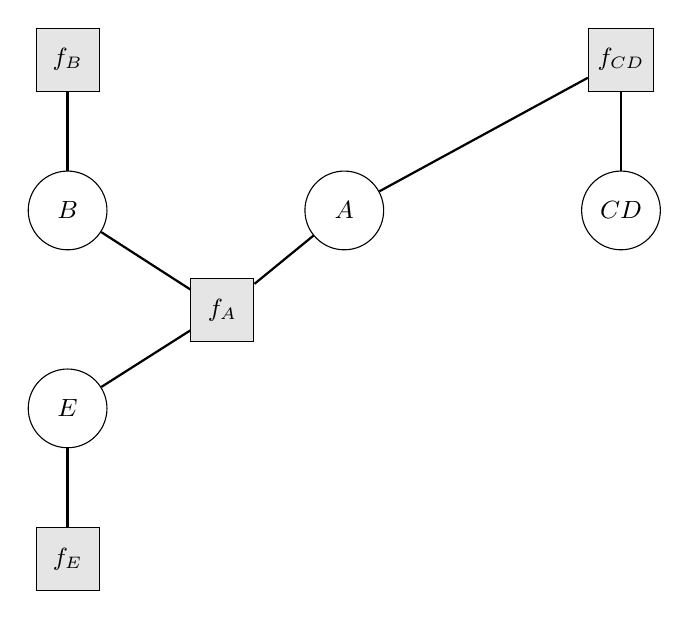
\begin{tikzpicture}[
  var/.style={circle, draw, minimum size=10mm, font=\small},
  fac/.style={rectangle, draw, fill=gray!20, minimum size=8mm, font=\small},
  edge/.style={thick},
  node distance=18mm
]
  \node[var] (B) {$B$};
  \node[var, right=25mm of B] (A) {$A$};
  \node[var, below=15mm of B] (E) {$E$};
  \node[var, right=25mm of A] (CD) {$CD$};
  \node[fac, above=10mm of B] (fB) {$f_B$};
  \node[fac, below=10mm of E] (fE) {$f_E$};
  \node[fac, below right=5mm and 12mm of B] (fA) {$f_A$};
  \node[fac, above=10mm of CD] (fCD) {$f_{CD}$};
  \draw[edge] (B) -- (fB);
  \draw[edge] (E) -- (fE);
  \draw[edge] (B) -- (fA);
  \draw[edge] (E) -- (fA);
  \draw[edge] (A) -- (fA);
  \draw[edge] (A) -- (fCD);
  \draw[edge] (CD) -- (fCD);
\end{tikzpicture}
\end{center}

\subsection{Credal Factors}

\paragraph{Factor $f_B$: $K(B)$.} Two vertices: $v_1 = [0.80, 0.20]$, $v_2 = [0.90, 0.10]$.

\paragraph{Factor $f_E$: $K(E)$.} Two vertices: $v_1 = [0.90, 0.10]$, $v_2 = [0.95, 0.05]$.

\paragraph{Factor $f_A$: $K(A \mid B, E)$.} Four parent configs, 2 vertices each:
\begin{center}
\begin{tabular}{llcc}
\toprule
\textbf{Config} & \textbf{Vtx} & $P(A{=}0)$ & $P(A{=}1)$ \\
\midrule
$B{=}0, E{=}0$ & $v_1$ & 0.9556 & 0.0444 \\
$B{=}0, E{=}0$ & $v_2$ & 1.0000 & 0.0000 \\
\midrule
$B{=}1, E{=}0$ & $v_1$ & 0.0000 & 1.0000 \\
$B{=}1, E{=}0$ & $v_2$ & 1.0000 & 0.0000 \\
\midrule
$B{=}0, E{=}1$ & $v_1$ & 0.0000 & 1.0000 \\
$B{=}0, E{=}1$ & $v_2$ & 1.0000 & 0.0000 \\
\midrule
$B{=}1, E{=}1$ & $v_1$ & 0.0000 & 1.0000 \\
$B{=}1, E{=}1$ & $v_2$ & 1.0000 & 0.0000 \\
\bottomrule
\end{tabular}
\end{center}

\paragraph{Factor $f_{CD}$: $K(CD \mid A)$.} $A{=}0$: 4 vertices; $A{=}1$: 11 vertices.
First two vertices of each:
\begin{center}
\begin{tabular}{llcccc}
\toprule
\textbf{Config} & \textbf{Vtx} & $P(0)$ & $P(1)$ & $P(2)$ & $P(3)$ \\
\midrule
$A{=}0$ & $v_1$ & 0.00 & 0.00 & 0.00 & 1.00 \\
$A{=}0$ & $v_2$ & 0.00 & 0.00 & 1.00 & 0.00 \\
\midrule
$A{=}1$ & $v_1$ & 0.00 & 0.00 & 0.30 & 0.70 \\
$A{=}1$ & $v_2$ & 0.00 & 0.30 & 0.00 & 0.70 \\
\bottomrule
\end{tabular}
\end{center}

\subsection{Query: $P(B{=}1)$, No Evidence}

\subsubsection{Global Vertex Combination 1: All $v_1$}

The global vc selects $v_1$ for every factor and every parent configuration.
This fixes a precise BN:
\[
  P(B) = [0.80, 0.20], \quad P(E) = [0.90, 0.10],
\]
\[
  P(A \mid B{=}0, E{=}0) = [0.9556, 0.0444], \quad
  P(A \mid \text{others}) = [0.0, 1.0],
\]
\[
  P(CD \mid A{=}0) = [0, 0, 0, 1], \quad P(CD \mid A{=}1) = [0, 0, 0.3, 0.7].
\]

\paragraph{Initialization.}
$q(B) = [0.5, 0.5]$, $q(E) = [0.5, 0.5]$, $q(A) = [0.5, 0.5]$,
$q(CD) = [0.25, 0.25, 0.25, 0.25]$.

\paragraph{Iteration 0: Update $q(B)$.}
Variable $B$ appears in two factors: $f_B$ (as child) and $f_A$ (as parent of $A$).

\textbf{Case 1} --- contribution from $f_B$ (child):
using Eq.~\eqref{eq:case1} with no parents:
\[
  \log \tilde{q}(B{=}0) \mathrel{+}= \log 0.80 = -0.2231, \qquad
  \log \tilde{q}(B{=}1) \mathrel{+}= \log 0.20 = -1.6094.
\]

\textbf{Case 2} --- contribution from $f_A$ ($B$ is parent of $A$):
using Eq.~\eqref{eq:case2}, summing over parent configs $\pi$ where $\pi_B = b$:
\begin{align*}
  \log \tilde{q}(B{=}0) &\mathrel{+}=
    q(E{=}0) \cdot \bigl[q(A{=}0) \log P(A{=}0 \mid 0,0) + q(A{=}1) \log P(A{=}1 \mid 0,0)\bigr] \\
    &\quad + q(E{=}1) \cdot \bigl[q(A{=}0) \log P(A{=}0 \mid 0,1) + q(A{=}1) \log P(A{=}1 \mid 0,1)\bigr] \\
  &= 0.5 \cdot [0.5 \cdot \log 0.9556 + 0.5 \cdot \log 0.0444] \\
  &\quad + 0.5 \cdot [0.5 \cdot (-\infty) + 0.5 \cdot \log 1.0].
\end{align*}
Since $\log 0 = -\infty$, the term involving $P(A{=}0 \mid B{=}0, E{=}1) = 0$ drives
$\log \tilde{q}(B{=}0) \to -\infty$.

Similarly, $\log \tilde{q}(B{=}1)$ receives a $-\infty$ contribution from
$P(A{=}0 \mid B{=}1, E{=}0) = 0$. In practice, $\log(0)$ is replaced by
$\log(10^{-300}) \approx -690.8$.

After exponentiating and normalizing:
\[
  q(B) = [1.0000,\; 0.0000].
\]
The zero CPT entries cause extreme variational updates that push $q(B)$ to a
degenerate distribution.

\paragraph{Update $q(E)$.} Analogous computation yields $q(E) = [1.0000, 0.0000]$.

\paragraph{Update $q(A)$.}
With $q(B) = [1.0, 0.0]$ and $q(E) = [1.0, 0.0]$, only the parent config $(B{=}0, E{=}0)$ has
nonzero weight:
\begin{align*}
  \log \tilde{q}(A{=}0) &\mathrel{+}= 1.0 \cdot 1.0 \cdot \log P(A{=}0 \mid 0,0) = \log 0.9556 = -0.0454, \\
  \log \tilde{q}(A{=}1) &\mathrel{+}= 1.0 \cdot 1.0 \cdot \log P(A{=}1 \mid 0,0) = \log 0.0444 = -3.1147.
\end{align*}
Plus contributions from $f_{CD}$ (Case~2, $A$ is parent of $CD$).
After normalization: $q(A) = [0.0000,\; 1.0000]$ (driven by the $f_{CD}$ contribution
which penalizes $A{=}0$ due to the degenerate $P(CD \mid A{=}0) = [0,0,0,1]$).

\paragraph{Iteration 1.}
With the updated $q(A) \approx [0, 1]$, the $f_A$ contribution to $q(B)$ now
weights parent configs differently. The coordinate ascent produces:
\[
  q(B) = [0.1509,\; 0.8491], \quad q(E) = [0.8491,\; 0.1509].
\]
$q(A)$ remains $[0.0, 1.0]$.

\paragraph{Convergence.} After several more iterations:
\[
  q(B) \approx [0.238,\; 0.762], \quad q(E) \approx [0.811,\; 0.189], \quad
  q(A) = [0.0,\; 1.0].
\]

\textbf{Record:} $q(B{=}1) = 0.762$ for this vertex combination.

\subsubsection{Global Vertex Combination 2: All $v_2$}

Select $v_2$ for every factor. This fixes:
\[
  P(B) = [0.90, 0.10], \quad P(E) = [0.95, 0.05],
\]
\[
  P(A \mid \text{all configs}) = [1.0, 0.0], \quad
  P(CD \mid A{=}0) = [0, 0, 1, 0].
\]

Since $P(A{=}1 \mid \cdot) = 0$ for all parent configurations, the variational
update immediately yields $q(A) = [1.0, 0.0]$.
With no $-\infty$ log-terms for $B$ (since $P(A{=}0 \mid \cdot) = 1.0$
everywhere), $q(B)$ directly reflects $f_B$'s CPT:
\[
  q(B) = [0.9000,\; 0.1000], \quad q(E) = [0.9500,\; 0.0500].
\]
Convergence is immediate (1 iteration).

\textbf{Record:} $q(B{=}1) = 0.100$.

\subsubsection{Tracking Bounds Across Combinations}

After processing both vertex combinations:
\begin{align*}
  \underline{P}(B{=}1) &= \min(0.762,\; 0.100) = 0.100, \\
  \overline{P}(B{=}1) &= \max(0.762,\; 0.100) = 0.762.
\end{align*}

As more vertex combinations are explored (up to 500 sampled out of 2816 total),
the bounds continue to be refined. The final bounds depend on which extreme
distributions the sampling covers.

\subsection{Comparison}

\begin{center}
\begin{tabular}{lccc}
\toprule
\textbf{Query} & \textbf{Method} & $\underline{P}(B{=}1)$ & $\overline{P}(B{=}1)$ \\
\midrule
$P(B{=}1)$ & Exact VE & 0.1000 & 0.2000 \\
$P(B{=}1)$ & Interval BP & 0.1000 & 0.2000 \\
$P(B{=}1)$ & Variational (500) & $\leq$ 0.1000 & $\geq$ 0.2000 \\
\bottomrule
\end{tabular}
\end{center}

The variational bounds may be wider than VE because mean-field introduces a
factored approximation: the true posterior may exhibit dependencies between
variables that $q(\mathbf{X}) = \prod q_i(X_i)$ cannot capture. Additionally,
sampling may not cover all extremal vertex combinations. For small networks,
exact VE is preferred; the variational approach scales better to larger networks
where VE is intractable.

\section{Comparison with Other Methods}

\begin{center}
\begin{tabular}{lcccc}
\toprule
\textbf{Property} & \textbf{Exact VE} & \textbf{$\varepsilon$-VE} & \textbf{Interval BP} & \textbf{Variational} \\
\midrule
Exact & Yes & No & No & No \\
Bound type & Tight & Outer & Outer & Inner/Outer \\
Multi-valued & Yes & Yes & Yes & Yes \\
Scalability & Low & Medium & High & Medium \\
\bottomrule
\end{tabular}
\end{center}

\section{Complexity}

For each vertex combination, one round of mean-field coordinate ascent takes
$O(n \cdot k \cdot S_{\max} \cdot k^{S_{\max}})$ time, where $n$ is the number of
variables, $k$ is the maximum domain size, and $S_{\max}$ is the maximum factor
scope size. With $T$ iterations per combination and $M$ sampled combinations, the
total complexity is $O(M \cdot T \cdot n \cdot k^{S_{\max}+1})$.

\section{References}

\begin{enumerate}
\item M.I.\ Jordan, Z.\ Ghahramani, T.S.\ Jaakkola, L.K.\ Saul. An introduction to
      variational methods for graphical models. \emph{Machine Learning}, 37:183--233, 1999.
\item J.S.\ Ide, F.G.\ Cozman. Approximate algorithms for credal networks with binary
      variables. \emph{IJAR}, 48(1):275--296, 2008.
\item A.\ Antonucci, C.P.\ de Campos, D.\ Huber, M.\ Zaffalon. Approximate credal
      network updating by linear programming. \emph{IJAR}, 58:25--38, 2015.
\item D.D.\ Mau\'a, F.G.\ Cozman. Thirty years of credal networks. \emph{IJAR},
      126:133--157, 2020.
\end{enumerate}

\end{document}
